%FF制御
本章では,マルチサイクルテストにおける故障検出能力低下問題への対策として,
FF制御点挿入技術(FF-CPI)について述べる.

%1節
\section{故障検出能力低下問題への対策}
3章で説明したように,マルチサイクルテストでは,キャプチャサイクルの増加に伴い,
被検査回路の内部状態遷移が低減し,新たな故障の検出が困難になる問題がある.
この対策として,文献[5]では,
FFの出力に値を強制的に遷移させる制御ポイント(CP)を挿入するFF-CPI技術が提案された.
制御ポイント挿入技術とは,被検査回路の内部状態遷移の低減によって
故障信号の伝搬や励起を阻害しているFFに,直接論理値を割り当てる技術である.
FFにCPを挿入することで,制御後のサイクルにおける
キャプチャパターンのランダム性を向上させることができる.
固定値0/1が印加される箇所に対して,制御した論理値1/0を割り当てることにより,
故障の励起を促し,故障検出能力の向上を期待する.

%2節
\section{FFCP回路構造}
本研究では,FFトグリング制御を用いる.
トグリング制御の制御モデルを図4.1に示す.

\begin{figure}[h]
    \begin{center}
        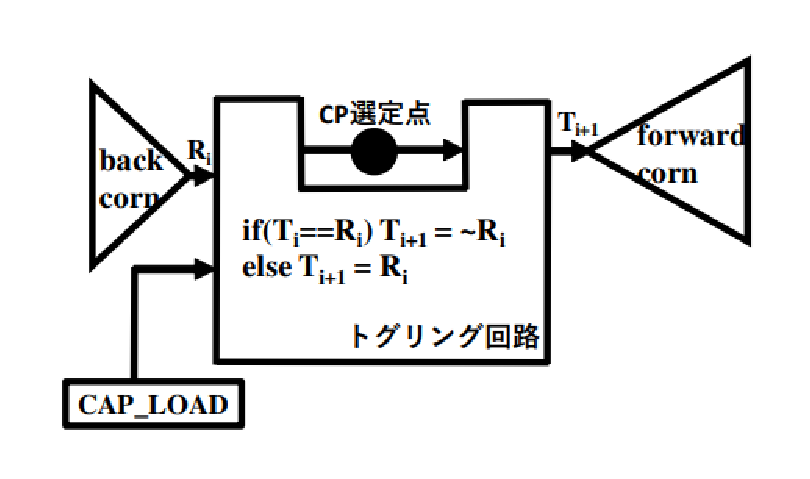
\includegraphics[height=50mm]{tgl.eps}
        \caption{トグリング制御モデル}
    \end{center}
\end{figure}

トグリング制御とは,選定した信号線にトグル回路を追加することで,
サイクル毎に選定信号線の値をトグルさせる手法である.
キャプチャモードでは,現在の状態(Ti:現在のキャプチャサイクルで適用されたテストパターン)と,
次の状態(Ri:現在のキャプチャサイクルで適用されたテストパターンのレスポンス)を比較して,
FFの値が変化しているかを確認する.変化していない場合は,
トグル制御回路はTi+1にトグルを生成し,Riの反転値を次のサイクルに伝搬させ,
変化している場合は,ば次のサイクルに現在のRiを伝搬させる.

また,本実験では,FF制御箇所はランダムに選定する.
